\phantomsection
\chapter{Conclusion}
\label{chap:ccl}
  
\phantomsection
\section{Theoretical framework}

\vspace{\baselineskip}
\noindent bla bla bla
\newline

\phantomsection
\section{Results}

\vspace{\baselineskip}
\noindent bla bla bla
\newline

\phantomsection
\section{Improvements}

\subsection{Local Binary Patterns}

\vspace{\baselineskip}
\noindent One of the way to improve the LBP operator of this system is to add weights for each of the 42 regions of the face as seen in chapter~\ref{chap:lbp}. The LBP operator used in this system has already some improvements; it is a uniform circular LBP operator. The results obtained with this operator are quite good with an accuracy of $ 61.90\% $. But this percentage of accuracy can be improved. Weighting the regions of the face is to have the most important features have more weight in the computation of the histograms.
\newline

\noindent The face image is divided in 42 regions ($ 6 $ columns $ \times $ $ 7 $ rows) as seen in chapter~\ref{chap:lbp}. The weights are however not applied in the same way. The Figure~\ref{lbp_region_weight} given in the chapter~\ref{chap:lbp} shows a face image containing only the face. The face images from the KDEF database on which this system is based are not the same. The face image contains also some background around the face. Thus, the regions that are at the border of the image and that represent the background have less weight than the one containing the face. The Figure~\ref{implementation_weight_example} shows an example of the division into regions of face images from the KDEF database that this system uses.
\newline

\begin{figure}[!h]
\begin{center}
\noindent 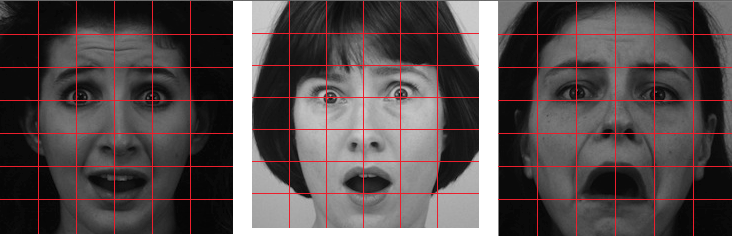
\includegraphics[scale=0.3]{figures/implementation_weight_example} 
\newline
\caption{Example of the division into regions of face images from the KDEF database}
\label{implementation_weight_example}
\end{center} 
\end{figure}

\noindent The weights assigned to this division of face are thus adapted. The weights are not the same that in the Figure~\ref{lbp_region_weight} given in the chapter~\ref{chap:lbp}. The weights are assigned as in the Figure~\ref{implementation_lbp_weight}. As it is shown in the Figure~\ref{implementation_lbp_weight}, the borderline weights are all of 1. It is because these regions are the background and do not have importance into the facial expression recognition system. All the weights of the regions characterizing the face are superior or equal to 2. The regions that have the highest weights are the region of the eyes and of the mouth.
\newline

\begin{figure}[!h]
\begin{center}
\noindent 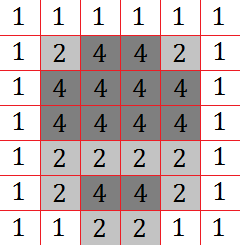
\includegraphics[scale=0.7]{figures/implementation_lbp_weight} 
\newline
\caption{Weights assignment used in this system}
\label{implementation_lbp_weight}
\end{center} 
\end{figure}

\noindent GIVE RESULTS WITH WEIGHTS APPLIED
\newline

\noindent Another way to improve the LBP operator would be to use one with larger scale; for example, $ LBP_{12,2.5}^{u^2} $ or $ LBP_{16,4.0}^{u^2} $ (with $ P = 12 $ and $ R = 2.5 $ or with $ P = 16 $ and $ R = 4.0 $). This implies to use the bilinear interpolation because the sampling points does not fall exactly on a pixel as seen in chapter~\ref{chap:lbp}. An using bilinear interpolation add sue more computation time. So it is more about finding a good compromise between computation time and accuracy for this system.
\newline

\subsection{Combination of feature extraction methods}

\vspace{\baselineskip}
\noindent To improve the accuracy of the feature extraction method that is LBP, another method of feature extraction can be used and combined with the one already used. 
\newline

\noindent  Here, for example, the LBP method has been combined with the Gabor filter one and it gives good results. This new method has been proposed by Liao et al. \cite{LIA09}. It is called the Dominant Local Binary Patterns (DLBP). It is robust against change of lightning, image rotation and about noise in the image.  It works by using the most recurrent patterns of the LBP method to obtain more information of the texture. It uses the Gabor method to add global texture information to the texture information already obtained by the LBP method. It works based on the circularly symmetric Gabor filter responses; this is the additional feature used with the LBP one \cite{LIA09}. Figure~\ref{combination_lbp_gabor} shows the robustness of the combination against change in lightning. The figure contains two face images of the YaleB face database. The (a) image is the original image with different lightnings. The (b) image is the preprocessed image with the gabor wavelets. The (c) image is the image mapped with the LBP operator. The (d) image is the preprocessed image with the combination of the two \cite{GOH11}.
\newline

\begin{figure}[!h]
\begin{center}
\noindent 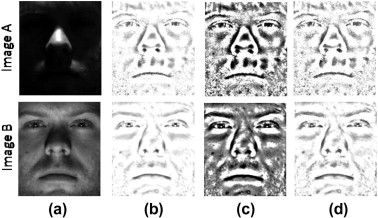
\includegraphics[scale=1]{figures/combination_lbp_gabor} 
\newline
\caption{2 face images of the YaleB face database}
\label{combination_lbp_gabor}
\end{center} 
\end{figure}

\noindent  LBP has also been combined with the Scale Invariant Feature Transform (SIFT). The SIFT descriptor is a descriptor of region of interest. This descriptor is robust against image rotation, image translations, scaling and variations in the lightning. Heikkila et al. introduced a combination of the SIFT descriptor with the LBP operator \cite{HEI09}.
\newline
